\renewcommand\evenpagerightmark{{\scshape\small The diffusion flame length prediction}}
\chapter[The diffusion flame length prediction]%
{The diffusion flame length prediction}
\label{The diffusion flame length prediction}
\section{An extensive review of the diffusion flame length formula }

Here is the list of all the formulas that I have found to predict a diffusion flame length. Though they seem very different, a detailed analysis will then show that they share many common features.

It is of importance to understand their origins, they can have three origins :
\begin{itemize}
\item analytical solution thanks to simplifications of the mechanisms
\item academic experiments in laboratory
\item industrial reports 
\end{itemize}

The used parameters will not be the same in the different cases, but it is very interesting to compare them.

\subsection{Laminar regime}
In a the laminar case : in (\# ref Veynante), the length of a diffusion flame in the laminar case is 
\begin{equation} \label{eq:length_laminar}
\frac{L_{f}}{e_{0}}=\frac{Re}{2\pi}\cdot \frac{1}{Z_{st}^2}
\end{equation}

  Though the regime is not of interest for industrial considerations, this formula con be demonstrated with medium effort, and permits to understand the most important parameters that drives the diffusion flame topology : the stoichiometric mixture fraction $Z_{st}$.
  \begin{equation}
Z_{st}=(1+\frac{\nu Y_{F,1}}{Y_{O_{2},2}})^{-1}
\end{equation}
  where $\nu$ is the mass stoechiometric ratio (4 for $CH_{4}-O_{2}$ flame),    $Y_{F,1}$ the mass ratio of fuel in the fuel injection ($Y_{F,1}=1$ if it is pure $CH_{4}$) and $Y_{O_{2},2}$ the mass ratio of oxygen in the oxidant injection ($Y_{O_{2},2}=0.23$ if it is pure air). One understands here that the stoichiometric mixture fraction is completely independent of the speeds, the mass flow, the bulk flow and the geometry. $Z_{st}$ only describes the composition of the gas. 

\subsection{Turbulent regime}

\subsubsection{Analysis from Peters  \cite{peters_four_1997}}
The analysis of Peters comes from the scenario of a fuel jet in a fixed oxidant :
\begin{equation}\label{eq: L_Peters}
\frac{L+x_{0}}{d}=\frac{2.19 (1+2Sc)}{Z_{st}}\frac{\rho_{0}}{\rho_{st}C}
\end{equation}

Where $Sc$  is the fixed turbulent Schmidt, $C$ the Chapman-Rubesin parameter, $\rho_{0}$ is the density at the nozzle and $\rho_{st}$ the density at the stoichiometry. $d$ is the diameter of the nozzle and $x_{0}$ the flame liftoff.

What mostly matters here is the stoichiometric mixture fraction still appears, and that $L$ depends on $\frac{1}{Z_{st}}$ in the turbulent case instead of $\frac{1}{Z_{st}^2}$ as it is the case in laminar regime.

It will be seen that this dependency on $\frac{1}{Z_{st}}$ is the characteristic of a diffusion turbulent flame.

\subsubsection{Experiment from Hawthorne \cite{hawthorne_mixing_????}}



Hawthorne gets experimentally the length  :
\begin{equation}\label{eq :L_hawthorne}
\frac{L+x_{0}}{d}=\frac{5.3}{Z_{st}}(\frac{\rho_{0}}{\rho_{st}})^{-1/2}
\end{equation}
Since it is quite close to Peters analysis \ref{eq: L_Peters}, Peters chose to fix in his formula $Sc$ and $C$ in order to fit to Hawthorne formula.

\paragraph{Numerical application} For a methane/air flame, we have $Z_{st}=(1+4\frac{1}{0.233})^{-1}=0.055$. Assuming $T_{st}=2000K$, it goes $\frac{\rho_{0}}{\rho_{st}}\sim 3.8$ and $L \sim 200d$.


\subsubsection{IFRF Online Combustion Handbook (industrial formula)\cite{neil_fricker_ifrf_2001}}

Here is the length $x_{s}$ where a jet can reach the stoichiometric equilibrium without combustion. We are now in an industrial case and not in the academic area :

\begin{equation}
x_{s}=5.9\Phi (1+\frac{V_{a}}{d_{g}})
\end{equation} with $\Phi=2\frac{Q_{m}}{\sqrt[]{\pi G \rho_{f}}}$. It can be noted that the notations are much more "industrial" :
\begin{itemize}
\item $V_{a}$ is "Stoichiometric Air Requirement (or Air Requirement) - The quantity of air required to completely combust a given quantity of a fuel - may be expressed on a volume or a mass or a mixed volume/mass basis (Vol/Vol)"
\item $d_{g}$ is the specific gravity of the fuel (density with respect to air)
\item $Q_{m}$ is the mass flow of fuel gas (kg/s)
\item $\rho_{f}$ is the density of the combustion products in the flame (kg/m3)
\item $G$ is the thrust of the incoming fuel jet (N)
\end{itemize}

It seems that this formula is completely new uncorrelated from the previous ones, however, using :
$Q_{air}\rho_{air}= \dot{m}_{air}$ and $Q_{fuel}\rho_{fuel}= \dot{m}_{fuel}$  ($Q$ being the bulk flow), we get :

\begin{equation}
V_{a}=\frac{Q_{air}}{Q_{fuel}}=\frac{ \dot{m}_{air}}{ \dot{m}_{fuel}}d_{g}
\end{equation}
Hence, using $\dot{m}_{CH_{4}}=Y_{1,CH_{4}}\cdot \dot{m}_{fuel}$and $\dot{m}_{O_{2}}=Y_{2,O_{2}}\cdot \dot{m}_{air}$
\begin{equation}
1+\frac{V_{a}}{d_{g}}=1+\frac{ \dot{m}_{air}}{ \dot{m}_{fuel}}=1+\frac{\nu Y_{F,1}}{Y_{O_{2},2}}=\frac{1}{Z_{st}}
\end{equation}

Consequently, it has been found that the industrial flame length formula also depends on $\frac{1}{Z_{st}}$ .

Using :
\begin{itemize}
\item $G=\dot m_{fuel} v_{fuel}$
\item $\dot m_{fuel}= v_{fuel} \cdot S_{fuel} \cdot \rho_{fresh fuel}$
\end{itemize}

And making the correspondence between the industrial and academic notations :
\begin{itemize}
\item $\rho_{fresh fuel}= \rho_{0} $
\item $\rho_{f}=\rho_{st}$
\item $Q_{m}=\dot{m}_{fuel}$
\end{itemize}
It goes :

\begin{equation}
\frac{x_{s}}{d}=5.92\frac{2Q_{m}}{\sqrt[]{\pi G \rho_{f}}}\frac{1}{Z_{st}}=\frac{5.92}{Z_{st}}(\frac{\rho_{0}}{\rho_{st}})^{1/2}
\end{equation} 
The formula is exactly the same as the one of Peters, except the factor.

The purpose of these formulas is obviously not to use them for a much more complicated case (swirled coaxial flow), but to consider that all the parametric parameters studied in Optisos report can be gathered with adimensional number. If these formula were correct, the flame length should depend on the stoichiometric mixture fraction $Z_{st}$, since $Z_{st}$ keeps all the information of S/C dilution, burner load or pressure variation of density.

\section{Investigation on Optisos analysis }

\subsection{Context of the investigation}

Given the lack of experimental data, predicting the flame length of the ATR burner seems is very unreachable. The experiments on Freiberg HP-POX burner are almost our only contact with industrial real results of combustion process in ATR burner. Furthermore, a detailed campaign has been made with parametric studies of different inputs, such as the S/C ratio, the load variation or the Oxygen/NG velocity ratio. The chosen metric to investigate the flame topology here will be the flame length 

The conclusion of the report are that :
\begin{enumerate}
\item Changing the pressure of the ATR burner from 30 to 50 bars leads to small variation of the flame length
\item The S/C ratio is the parameter that the biggest impact on the flame topology : With a S/C ratio increasing from 1 to 1.4, the flame length decreases from 124mm to 84mm
\item The burner load also drives the flame length : increasing burner load shortens the flame
\item High temperatures of the reactor leads to longer flame
\end{enumerate}

In order to emphasize the conclusion of the reports, here are the corresponding plot from Optisos report :

\begin{figure}[h!]
  \centering
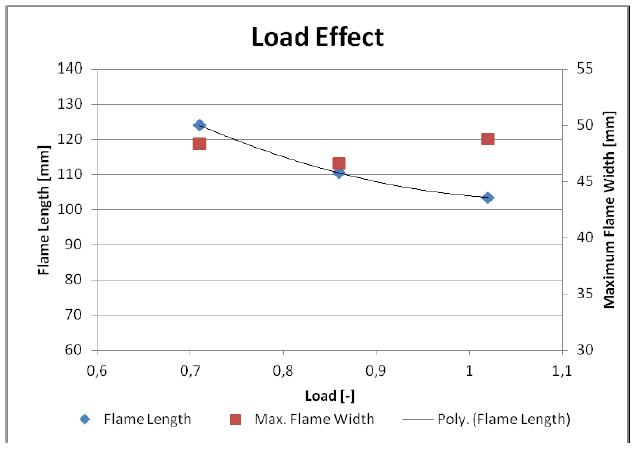
\includegraphics[width=0.45\textwidth]{fig/Optisos_Load_effect.PNG}
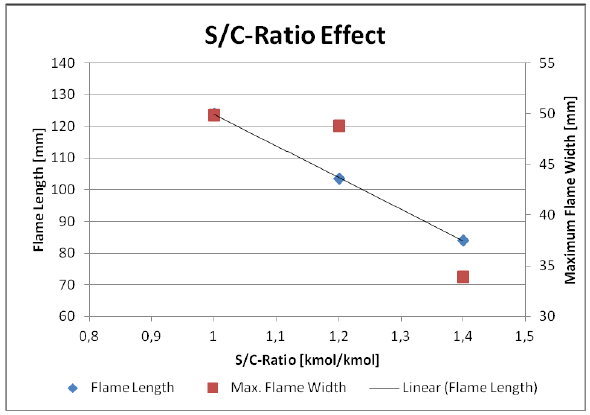
\includegraphics[width=0.45\textwidth]{fig/Optisos_S_C_effect.PNG}
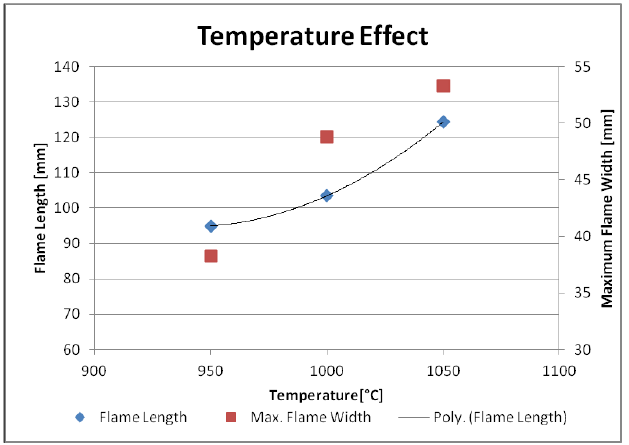
\includegraphics[width=0.45\textwidth]{fig/Optisos_temperature_effect.PNG}
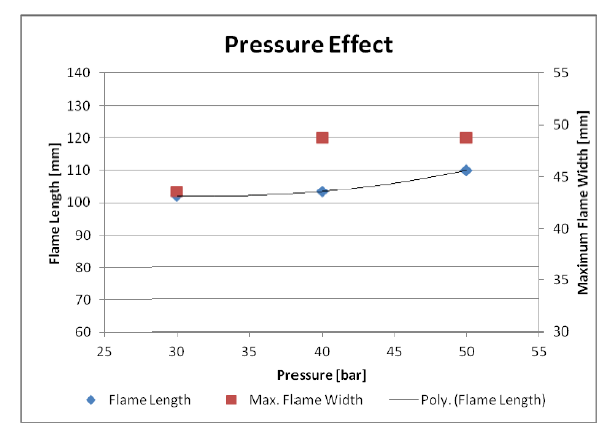
\includegraphics[width=0.45\textwidth]{fig/Optisos_Pressure_effect.PNG}
  \caption{Conclusion of Optisos report on flame topology}
 \label{optisos_plot}
\end{figure}

Dealing with my internship, if the flame length depended on so many parameters, it mean that I would have to study them all, and to keep them constant in Calhory burner with scales-up rule. This task seems impossible to achieve. Besides, a analysis of  the literature gives another interpretation. 



In this chapter, the data from Optisos has been re-used to compute in each test the corresponding $Z_{st}$, and it has be found that, in the area of the tests that have been conducted, the flame length of ATR burner measured in Optisos diagnostic directly depends on the stoichiometric mixture fraction $Z_st$ as an affine function :

The points in red are the cases where the temperature of the reactor has been changed, which does not implicate the $Z_{st}$, and adresses heat transfer and kinetic.

\begin{figure}[h!]
  \centering
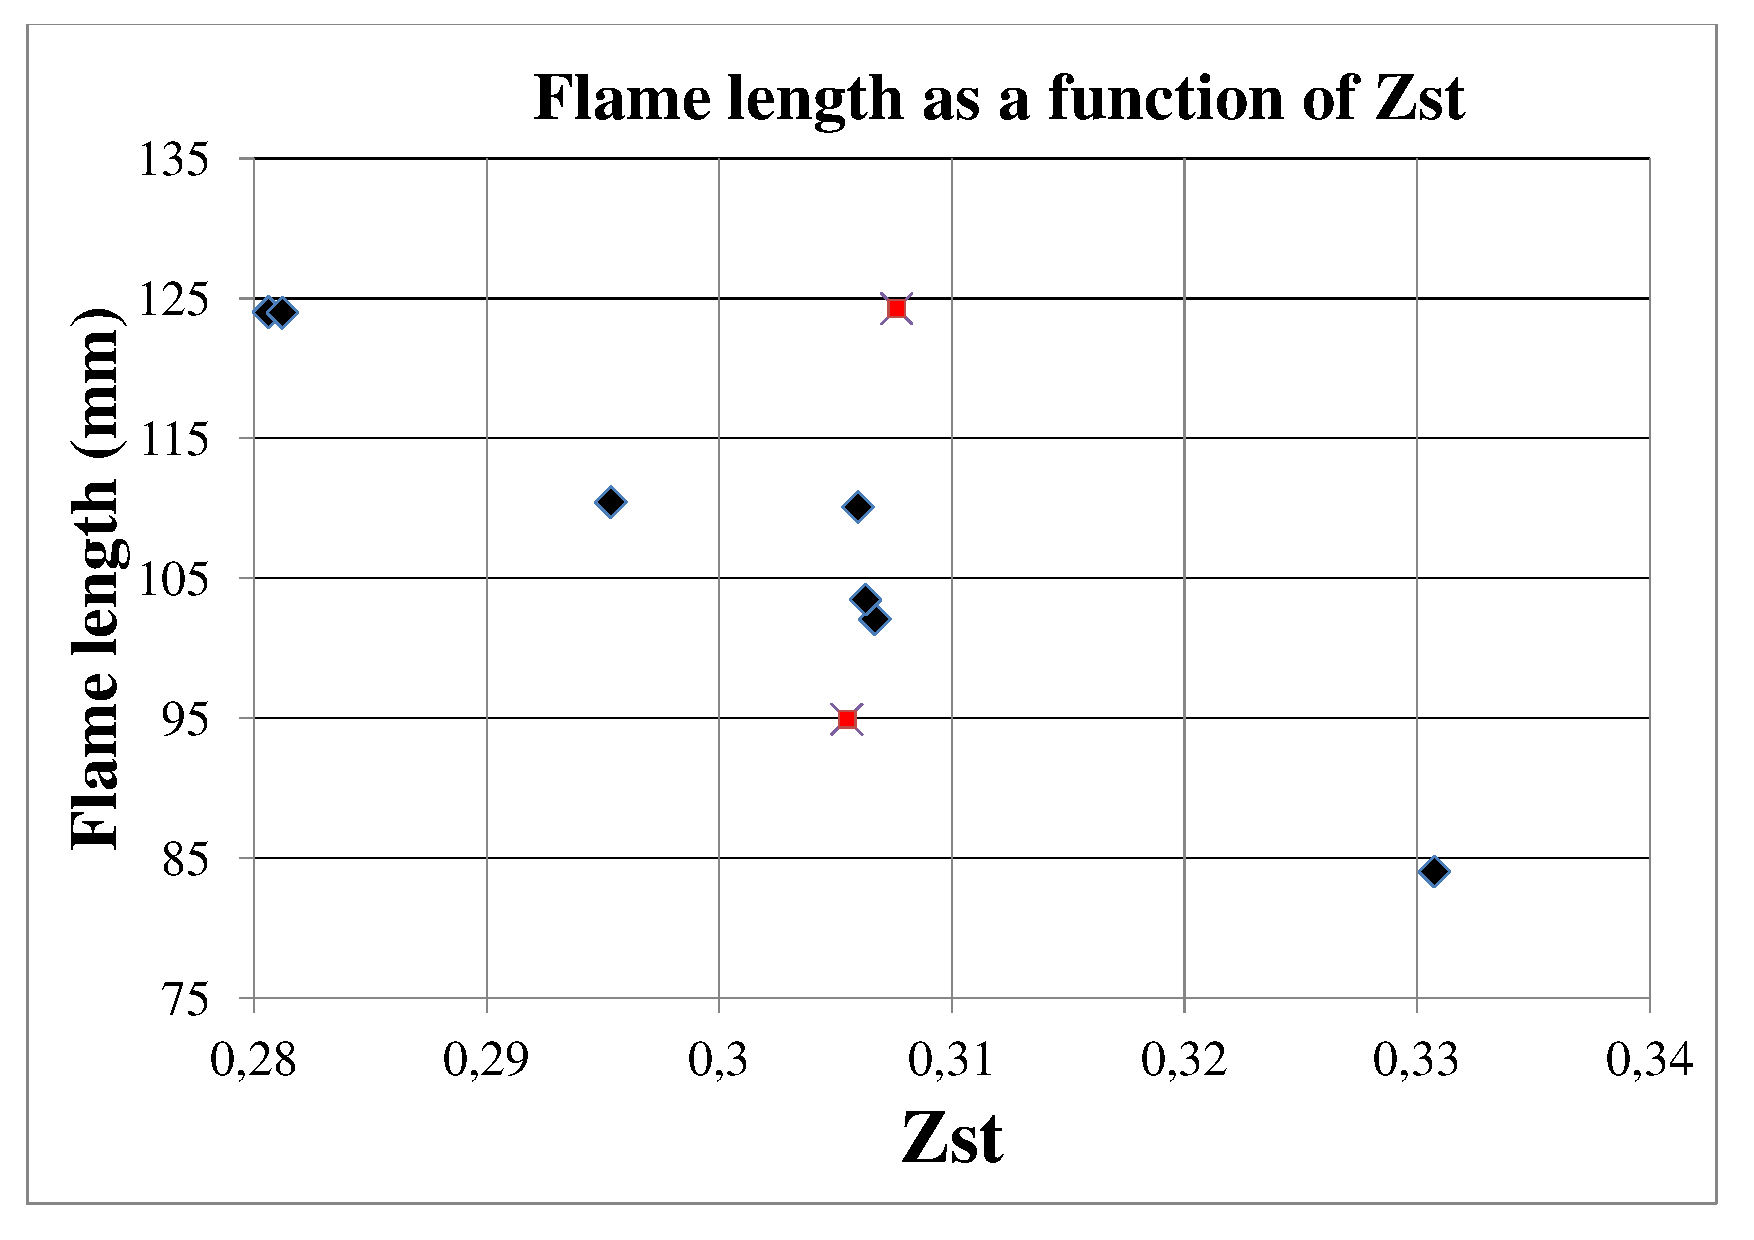
\includegraphics[width=0.8\textwidth]{fig/Flame_length_Zst.pdf}
 \label{Flame length as a function of Zst}
\end{figure}

It would be interested to get more points, or to extend the investigation segment, to define a characteristic law such as $Length=A_{0}-A_{1}\cdot Z_{st}$. One can easily verify that the trend is logical according to what have been observed previously, 